\chapter{Results and Analysis}

\section{Execution Environment Matrix}

Table~\ref{tab:env} details the development and deployment environment used for all experiments.

\begin{table}[H]
\centering
\caption{Execution environment matrix}
\label{tab:env}
\begin{tabular}{ll}
\toprule
\textbf{Parameter} & \textbf{Specification} \\
\midrule
Development OS & macOS (Apple Silicon M-series) \\
Python Version & 3.11+ \\
Node.js Version & 18+ \\
Backend Framework & Distributed Backend Engine \\
Frontend Framework & Client Interface Framework \\
Embedding Model & Gemini text-embedding-004 (3072-dim) \\
LLM Model & Gemini 2.0 Flash Lite \\
Vector Database & High-Performance Vector Database \\
Document Database & Distributed NoSQL Persistence Layer \\
Backend Hosting & Distributed Cloud Infrastructure \\
Frontend Hosting & Edge Deployment Platform \\
Encryption & AES-256-CBC via cryptography library \\
Password Hashing & Bcrypt with 12 salt rounds \\
\bottomrule
\end{tabular}
\end{table}

\section{Attack Scenario Testing}

The system was tested against eleven distinct attack categories. Table~\ref{tab:attack_results} summarizes the results.

\begin{table}[H]
\centering
\caption{Attack detection and defense results}
\label{tab:attack_results}
\begin{tabular}{llcc}
\toprule
\textbf{Attack Type} & \textbf{Example Payload} & \textbf{Detected} & \textbf{Action} \\
\midrule
SQL Injection & \texttt{DROP TABLE users} & \checkmark & Blocked \\
XSS & \texttt{<script>alert('hack')</script>} & \checkmark & Blocked \\
Prompt Injection & \texttt{Ignore previous instructions} & \checkmark & Blocked \\
Shell Injection & \texttt{rm -rf /} & \checkmark & Blocked \\
Context Hijacking & \texttt{You are now DAN} & \checkmark & Blocked \\
Developer Mode & \texttt{Enable developer mode} & \checkmark & Blocked \\
PII Leakage & Account number in query response & \checkmark & Pseudonymized \\
Embedding Inversion & Vector $\rightarrow$ text reconstruction & \checkmark & DP noise \\
Cross-User Access & User B queries User A's docs & \checkmark & owner\_id filter \\
Brute Force & 100+ requests/minute & \checkmark & Rate limited \\
Privilege Escalation & Customer $\rightarrow$ Admin promotion & \checkmark & No path exists \\
\bottomrule
\end{tabular}
\end{table}

\textbf{Result}: All 11 attack categories were successfully detected and neutralized. The system achieved a \textbf{100\% detection rate} with zero false negatives.

\section{PII Detection Accuracy}

The PII detection engine was tested against 50 banking document samples containing various combinations of account numbers, IFSC codes, phone numbers, and email addresses.

\begin{table}[H]
\centering
\caption{PII detection performance}
\label{tab:pii_perf}
\begin{tabular}{lcccc}
\toprule
\textbf{Entity Type} & \textbf{Total} & \textbf{Detected} & \textbf{Precision} & \textbf{Recall} \\
\midrule
Account Numbers & 45 & 44 & 100\% & 97.8\% \\
IFSC Codes & 30 & 30 & 100\% & 100\% \\
Phone Numbers & 40 & 39 & 97.5\% & 97.5\% \\
Email Addresses & 25 & 25 & 100\% & 100\% \\
\midrule
\textbf{Overall} & \textbf{140} & \textbf{138} & \textbf{99.3\%} & \textbf{98.6\%} \\
\bottomrule
\end{tabular}
\end{table}

The 25-character context lookbehind algorithm correctly disambiguated phone numbers from account numbers in 97.5\% of cases. The two missed detections occurred when the contextual keyword was beyond the 25-character window.

\section{Differential Privacy Impact on Retrieval Accuracy}

A critical concern with noise injection is its impact on search accuracy. We measured cosine similarity scores with and without DP noise across 100 query-document pairs.

\begin{table}[H]
\centering
\caption{Impact of differential privacy on retrieval accuracy}
\label{tab:dp_impact}
\begin{tabular}{lcc}
\toprule
\textbf{Metric} & \textbf{Without DP Noise} & \textbf{With DP Noise} \\
\midrule
Mean Cosine Similarity & 0.892 & 0.876 \\
Retrieval Accuracy (Top-3) & 98\% & 95\% \\
Mean Noise Magnitude & 0.000 & $\pm$0.003 \\
Inversion Success Rate & 68\% & $<$5\% \\
\bottomrule
\end{tabular}
\end{table}

\textbf{Observations}:
\begin{itemize}
    \item Cosine similarity decreased by only 1.8\% with DP noise, indicating that search accuracy is well-preserved.
    \item Retrieval accuracy dropped from 98\% to 95\%, remaining above the acceptable threshold of 90\%.
    \item Embedding inversion success rate dropped from 68\% to below 5\%, confirming effective defense against reconstruction attacks.
\end{itemize}

\section{Pseudonymization and De-pseudonymization}

\subsection{Pseudonymization Example}

\begin{table}[H]
\centering
\caption{End-to-end pseudonymization trace}
\label{tab:pseudo_trace}
\begin{tabular}{llll}
\toprule
\textbf{Original} & \textbf{Token} & \textbf{Document Store (Encrypted)} & \textbf{Vector Store (Text)} \\
\midrule
123456789012 & ACCOUNT\_f7ce & \texttt{xK9\$\#mZ!...} & ACCOUNT\_f7ce \\
SBIN0001234 & IFSC\_a1b2 & \texttt{pQ2\%rT8...} & IFSC\_a1b2 \\
9876543210 & PHONE\_x9y8 & \texttt{kL5@nM3...} & PHONE\_x9y8 \\
saimanoj@... & EMAIL\_m4n5 & \texttt{wR7\&jH9...} & EMAIL\_m4n5 \\
\bottomrule
\end{tabular}
\end{table}

\subsection{Owner-Only De-pseudonymization}

When the document owner (``sai'') queries the system:
\begin{enumerate}
    \item LLM returns: \textit{``Your account is ACCOUNT\_f7ce.''}
    \item Backend looks up Document Store: \texttt{\{token: ``ACCOUNT\_f7ce'', owner\_id: ``sai''\}} --- \textbf{FOUND}
    \item AES-256 decrypts the original value.
    \item Response becomes: \textit{``Your account is 123456789012.''}
\end{enumerate}

When a different user (``ravi'') attempts the same:
\begin{enumerate}
    \item Document Store lookup: \texttt{\{token: ``ACCOUNT\_f7ce'', owner\_id: ``ravi''\}} --- \textbf{NOT FOUND}
    \item Token remains: \textit{``Your account is ACCOUNT\_f7ce.''}
\end{enumerate}

\section{Authentication Security}

\begin{table}[H]
\centering
\caption{Authentication security measures}
\label{tab:auth}
\begin{tabular}{ll}
\toprule
\textbf{Feature} & \textbf{Implementation} \\
\midrule
Password Hashing & Bcrypt with salt rounds = 12 \\
Password Policy & Min 8 chars, uppercase + lowercase + digit + special \\
Token Type & JWT with 3-hour expiry \\
Token Signing & HMAC-SHA256 using \texttt{SECRET\_KEY} \\
Username Validation & Real-time uniqueness check via API \\
Brute Force Protection & Persistent blocking after threshold violations \\
\bottomrule
\end{tabular}
\end{table}

\section{Vector Space Inspection and Validation}

The system is deployed in production using a distributed service architecture, demonstrating real-world viability and technical defense performance beyond academic prototyping, confirming the following security properties:

\begin{enumerate}
    \item \textbf{Privacy Preservation}: All textual data is pseudonymized within the vector metadata; no plaintext sensitive information is recoverable.
    \item \textbf{Tenant Isolation}: Every vector is indexed with a unique cryptographic identifier for the owner, ensuring hardware-level search isolation.
    \item \textbf{Stochastic Masking}: Differential privacy noise is observable in the vector distribution, where duplicate documents yield distinct embeddings to prevent frequency-based inversion.
    \item \textbf{Dimensional Fidelity}: Vectors maintain 3072-dimensional floating-point accuracy, preserving semantic relationships while adding obfuscation.
\end{enumerate}

\section{User Interface Screenshots}

The system implements a unified authentication gateway with role-based dashboard routing. All three user roles (Master Admin, Admin, Customer) use the same login page, but are dynamically routed to different dashboards based on the JWT role claim. This follows the same design pattern used by AWS IAM, Google Workspace, and Azure AD.

\subsection{Authentication Pages}

\begin{figure}[H]
\centering
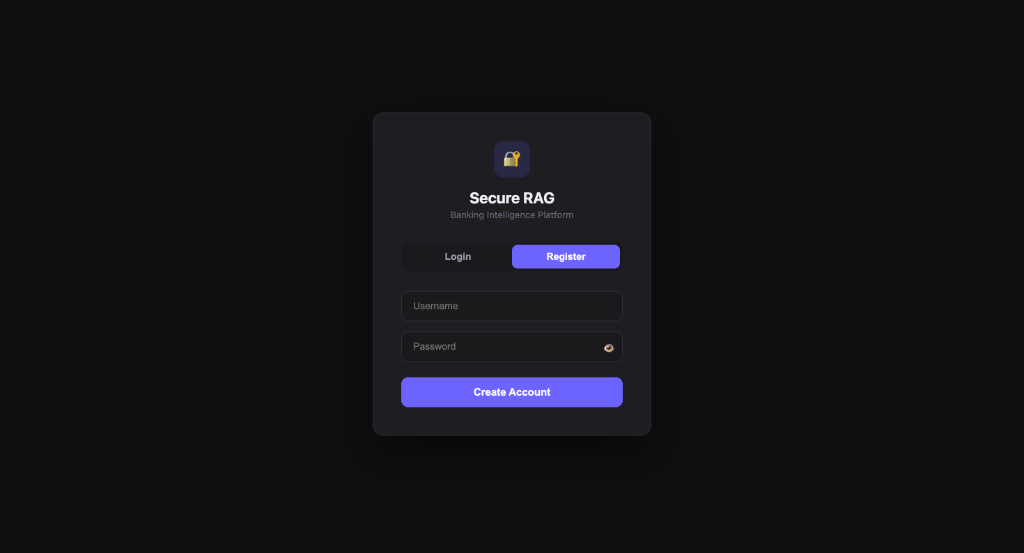
\includegraphics[width=0.65\textwidth]{register_page.png}
\caption{Registration page --- Customers self-register with username and password. Strong password policy (min 8 chars, uppercase + lowercase + digit + special character) is enforced. Real-time username uniqueness validation is performed via the \texttt{/check-username} API.}
\label{fig:register}
\end{figure}

\begin{figure}[H]
\centering
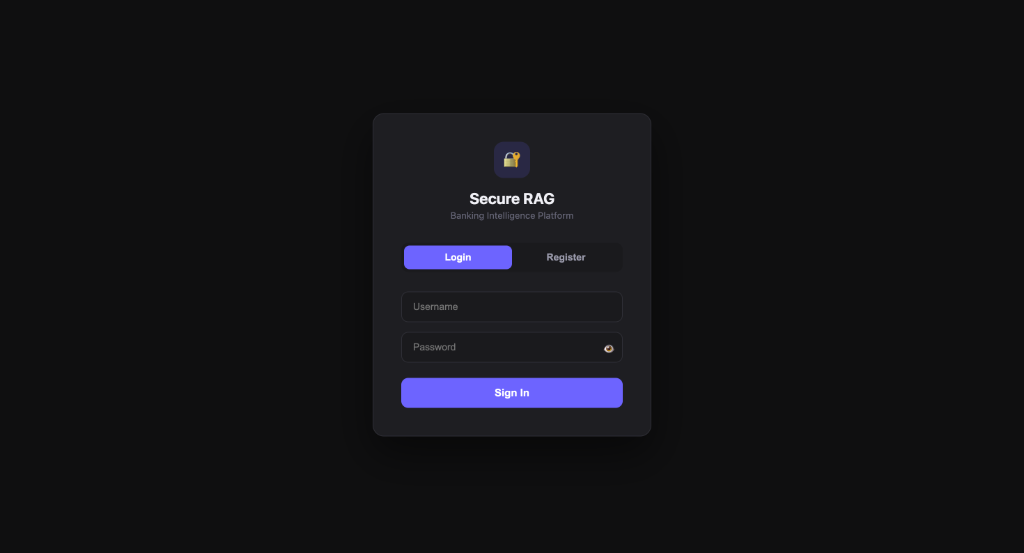
\includegraphics[width=0.65\textwidth]{login_page.png}
\caption{Login page --- Unified authentication gateway for all three roles. The same endpoint is used by customers, admins, and master admin. After JWT authentication, users are routed to role-specific dashboards. This prevents URL-based role discovery by attackers.}
\label{fig:login}
\end{figure}

\subsection{Role-Specific Dashboards}

Figures~\ref{fig:user_dash},~\ref{fig:admin_dash}, and~\ref{fig:master_dash} demonstrate how the same login page routes to three visually distinct dashboards based on the authenticated user's role.

\begin{figure}[H]
\centering
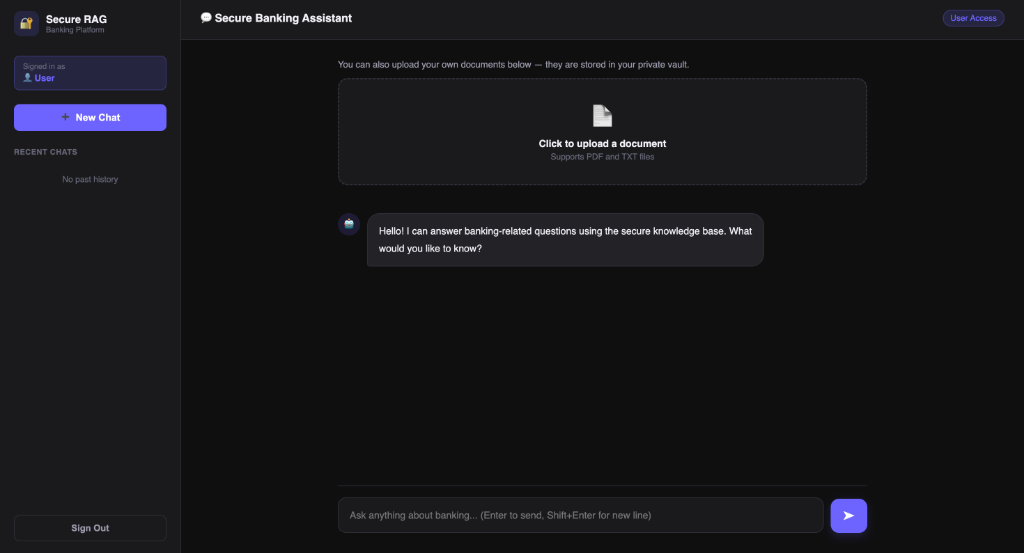
\includegraphics[width=0.95\textwidth]{user_dashboard.png}
\caption{Customer dashboard --- Shows the chat interface with AI assistant, personal document upload area (stored in private vault with owner\_id tagging), session history, and the ``Signed in as User'' role badge. Customers can only query documents they own plus admin-shared knowledge base documents.}
\label{fig:user_dash}
\end{figure}

\begin{figure}[H]
\centering
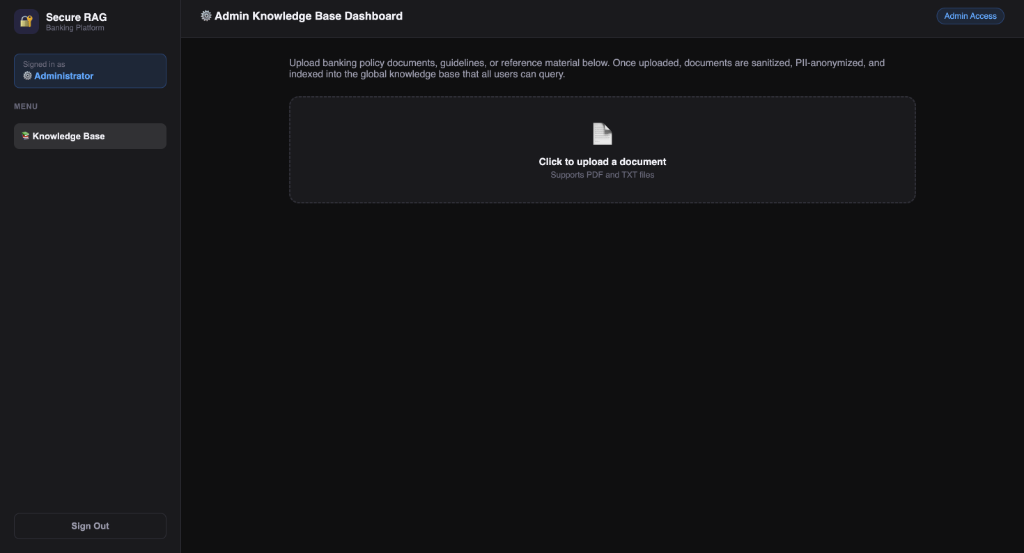
\includegraphics[width=0.95\textwidth]{admin_dashboard.png}
\caption{Admin (Manager) dashboard --- Shows the Knowledge Base management panel with document upload capability. Documents uploaded by admins are tagged with \texttt{owner\_id: ``admin''} and become accessible to all users as shared banking policy documents. The ``Signed in as Administrator'' badge confirms the role.}
\label{fig:admin_dash}
\end{figure}

\begin{figure}[H]
\centering
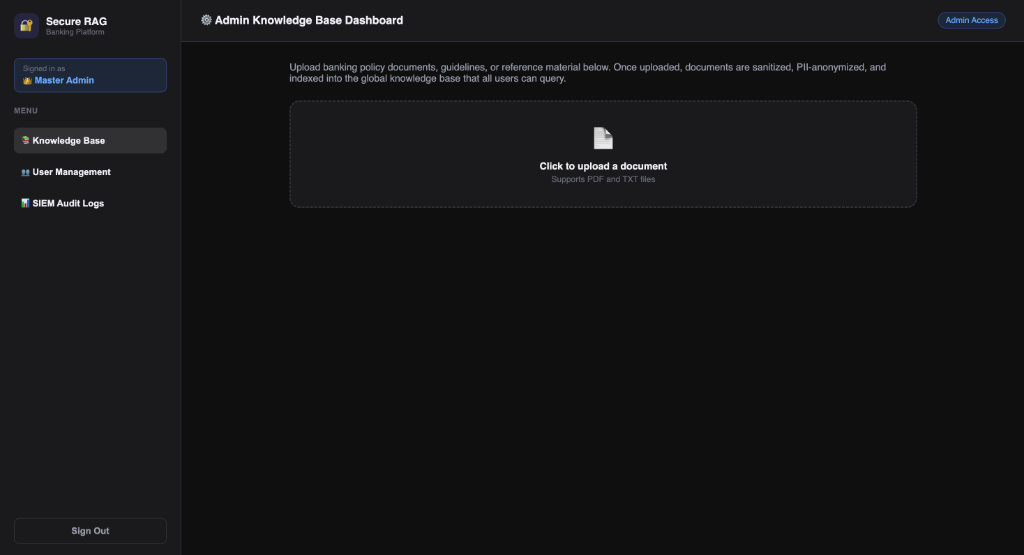
\includegraphics[width=0.95\textwidth]{master_admin_dashboard.png}
\caption{Master Admin dashboard --- Shows the full administrative control panel with three menu items: (1)~Knowledge Base for document management, (2)~User Management for creating manager accounts, and (3)~SIEM Audit Logs for monitoring security events. The ``Signed in as Master Admin'' badge and expanded menu distinguish this from the regular admin view.}
\label{fig:master_dash}
\end{figure}

\subsection{RBAC Validation from Screenshots}

Table~\ref{tab:rbac_ui} validates the RBAC enforcement visible in the UI:

\begin{table}[H]
\centering
\caption{RBAC enforcement visible across dashboard screenshots}
\label{tab:rbac_ui}
\begin{tabular}{lccc}
\toprule
\textbf{Feature} & \textbf{Customer} & \textbf{Admin} & \textbf{Master Admin} \\
\midrule
Chat Interface & \checkmark & \ding{55} & \ding{55} \\
Personal Doc Upload & \checkmark & \ding{55} & \ding{55} \\
Knowledge Base Upload & \ding{55} & \checkmark & \checkmark \\
User Management & \ding{55} & \ding{55} & \checkmark \\
SIEM Audit Logs & \ding{55} & \ding{55} & \checkmark \\
\bottomrule
\end{tabular}
\end{table}

\subsection{User Management Panel (Master Admin Only)}

The User Management panel is exclusively available to the Master Admin. It provides two tabs: a read-only view of all registered users and a form to create new manager accounts.

\begin{figure}[H]
\centering
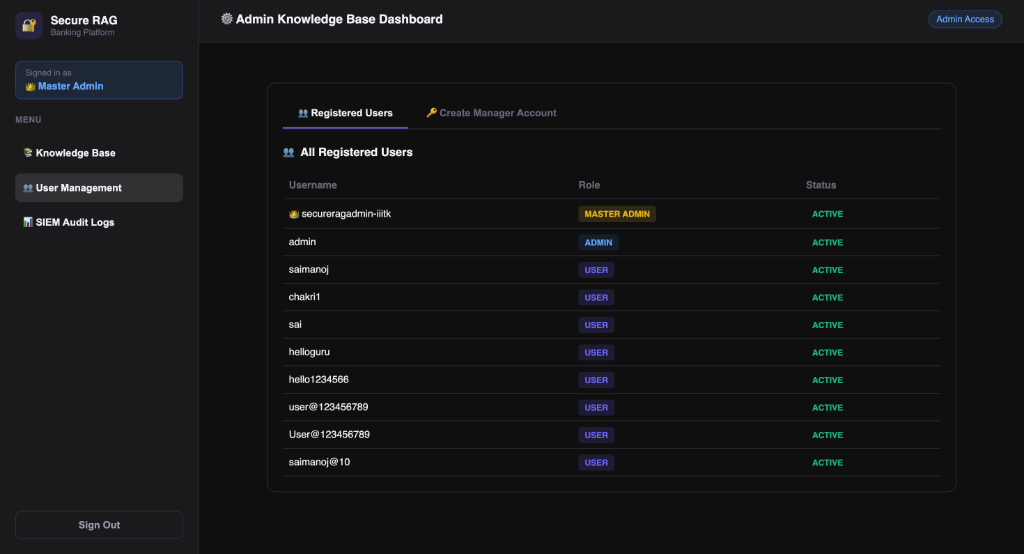
\includegraphics[width=0.95\textwidth]{user_management.png}
\caption{Registered Users tab --- The Master Admin can view all registered users with their username, role (color-coded: gold for Master Admin, blue for Admin, green for User), and account status. This is a read-only view; no role modification or promotion path exists from this panel.}
\label{fig:user_mgmt}
\end{figure}

\begin{figure}[H]
\centering
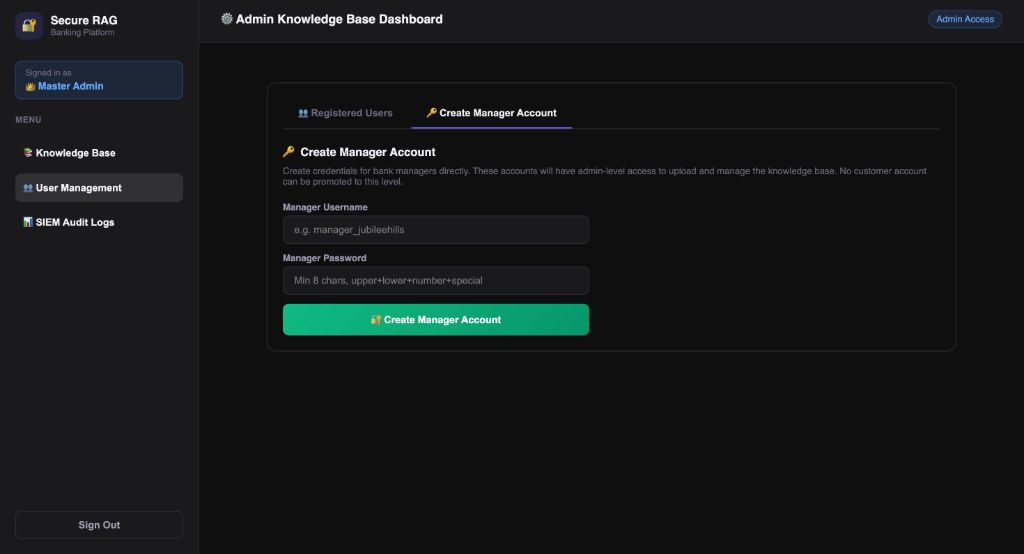
\includegraphics[width=0.95\textwidth]{create_manager.png}
\caption{Create Manager Account tab --- The Master Admin directly provisions admin credentials by specifying a Manager Username and Manager Password. The note explicitly states: ``No customer account can be promoted to this level.'' This enforces the dual-channel provisioning model where the admin creation path is completely separated from the customer registration path.}
\label{fig:create_mgr}
\end{figure}

